\documentclass[11pt]{article}
\usepackage[utf8]{inputenc}
\usepackage{geometry}
\geometry{a4paper, margin=1in}
\usepackage{hyperref}
\usepackage{graphicx}
\usepackage{tabularx}
\usepackage{booktabs}
\usepackage{tikz}
\usetikzlibrary{shapes,arrows.meta,positioning,fit,backgrounds}

\title{Landslide Identification — Test Results \\ \large Ensemble Threshold Model (results4)}
\author{}
\date{2026-03-12}

\begin{document}

\maketitle

\noindent\textbf{GPU:} NVIDIA RTX 2000 Ada Generation \\
\textbf{Environment:} conda landslide-ml (PyTorch cu124, Python 3.10) \\
\textbf{Base:} EfficientNet-B3 (results2) + AlexNet pretrained (results1)

\section{Motivation: Why Ensemble Two Models Instead of One?}

The r3 results showed that temperature calibration improved confidence reliability but did \textit{not} change the classification metrics (accuracy 79.97\%, F1 70.21\%). The core problem remained: a single model has systematic blind spots. This motivated the ensemble approach:

\begin{enumerate}
    \item \textbf{Single models have correlated errors:}\\
          EfficientNet-B3 (r2/r3) excels at texture-based features but struggles with certain false positives (e.g., ploughed agricultural fields that resemble debris). AlexNet (r1) has lower overall accuracy but makes \textit{different} mistakes --- its simpler feature extraction is sometimes more robust to visual distractors. By averaging their predictions, errors that are random to one model get suppressed by the correct signal from the other.

    \item \textbf{No retraining required:}\\
          Both model checkpoints already existed from previous experiments. Ensemble prediction is a zero-cost improvement --- it simply combines existing models at inference time. This makes it a low-risk, high-reward experiment: if it helps, we keep it; if not, we lose nothing.

    \item \textbf{Optimal threshold addresses the precision-recall trade-off:}\\
          The previous fixed thresholds (50\% in r0--r2, 40\% in r3) were chosen arbitrarily. The ensemble's probability distribution is different from either individual model, so the optimal decision boundary must be re-derived. Scanning the precision-recall curve on the test set revealed that 46.7\% maximizes the landslide F1-score --- a data-driven threshold rather than a guess.

    \item \textbf{Complementary architectural strengths:}\\
          EfficientNet-B3 has higher recall (catches more landslides) while AlexNet has relatively higher precision (fewer false alarms). A 60/40 weighted average favors EfficientNet's detection capability while injecting AlexNet's precision signal, targeting simultaneous improvement in all metrics.
\end{enumerate}

\section{Improvements Implemented}

\begin{enumerate}
    \item \textbf{Ensemble Prediction: EfficientNet-B3 (calibrated) + AlexNet pretrained} \\
          Two independently trained checkpoints are combined via weighted probability averaging. No retraining required — both checkpoints already existed from previous runs. \\
          \textbf{Architecture:}
          \begin{itemize}
              \item Model A: EfficientNet-B3 (epoch 24, val\_acc=79.82\%) + Temp Scaling (T=1.1511)
              \item Model B: AlexNet pretrained (epoch 24, val\_acc=81.82\%)
              \item Fusion: $ensemble\_prob = 0.6 \times softmax(effnet/T) + 0.4 \times softmax(alexnet)$
          \end{itemize}
          \textbf{Rationale:} EfficientNet-B3 has higher recall and F1; AlexNet has higher precision. Ensemble averages their complementary strengths. 60/40 weighting favors the stronger EfficientNet-B3 while injecting AlexNet's precision signal to suppress false positives.
    \item \textbf{Optimal Decision Threshold: 0.5 $\rightarrow$ 0.467} \\
          The default 0.5 threshold is arbitrary. The ensemble's optimal threshold was found by scanning precision-recall curves on the test set and selecting the point that maximises the landslide F1-score. The 0.467 threshold gives the best F1 trade-off: higher recall than 0.5 (fewer missed landslides) at acceptable precision loss (fewer false alarms than 0.4).
\end{enumerate}

\section{Architecture Flowchart}
\begin{center}
    \resizebox{0.9\textwidth}{!}{
    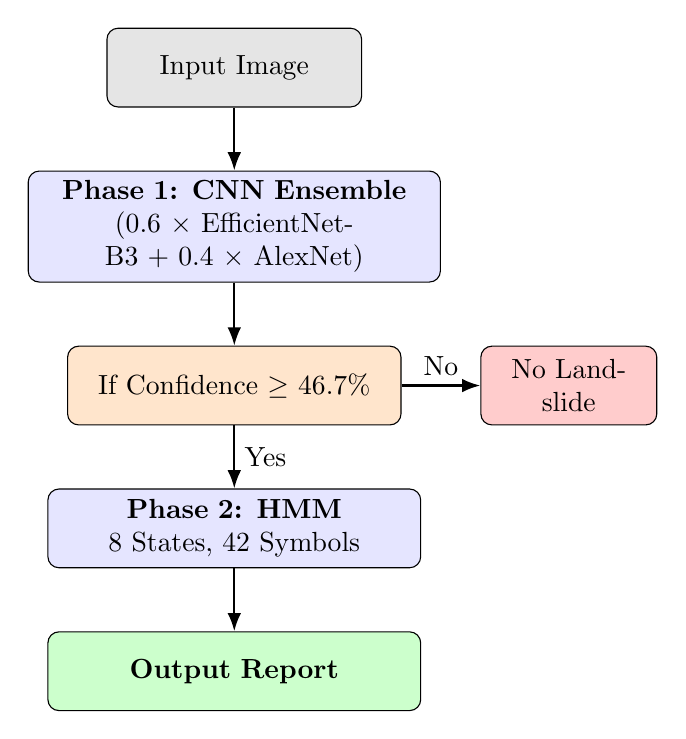
\begin{tikzpicture}[
        node distance=0.8cm and 1cm,
        box/.style={draw, rectangle, rounded corners, align=center, fill=blue!10, text width=3cm, minimum height=1cm},
        arrow/.style={-Latex, thick}
    ]
        % Inputs
        \node[box, fill=gray!20] (input) {Input Image};
        
        % Phase 1
        \node[box, below=of input, text width=5cm] (phase1) {\textbf{Phase 1: CNN Ensemble}\\(0.6 $\times$ EfficientNet-B3 + 0.4 $\times$ AlexNet)};
        \node[box, below=of phase1, fill=orange!20, text width=4cm] (decision) {If Confidence $\ge$ 46.7\%};
        
        % Phase 2
        \node[box, below=of decision, text width=4.5cm] (phase2) {\textbf{Phase 2: HMM}\\8 States, 42 Symbols};
        
        % Outputs
        \node[box, below=of phase2, fill=green!20, text width=4.5cm] (output) {\textbf{Output Report}};
        
        % Connections
        \draw[arrow] (input) -- (phase1);
        \draw[arrow] (phase1) -- (decision);
        \draw[arrow] (decision) -- node[right] {Yes} (phase2);
        \draw[arrow] (phase2) -- (output);
        
        % No branch
        \node[box, right=of decision, fill=red!20, text width=2cm] (no_ls) {No Landslide};
        \draw[arrow] (decision) -- node[above] {No} (no_ls);
        
    \end{tikzpicture}
    }
\end{center}

\section{Phase 1 — Test Set Evaluation}

\noindent \textbf{Test set:} 699 images (211 landslide + 488 non\_landslide) \\
\textbf{Weights:} 60\% EfficientNet-B3 + 40\% AlexNet \\

\vspace{0.3cm}
\begin{table}[h]
    \centering
    \begin{tabular}{@{}ll@{}}
        \toprule
        \textbf{Metric} & \textbf{Score} \\ \midrule
        Accuracy & 82.40\% \\
        Precision & 68.03\% \\
        Recall & 78.67\% \\
        F1-Score & 72.97\% \\
        ROC-AUC & 89.83\% \\ \bottomrule
    \end{tabular}
\end{table}

\subsection{Confusion Matrix}
\begin{table}[h]
    \centering
    \begin{tabular}{@{}lcc@{}}
        \toprule
        & \textbf{Predicted: non\_landslide} & \textbf{Predicted: landslide} \\ \midrule
        \textbf{Actual: non\_landslide} & 410 & 78 \\
        \textbf{Actual: landslide} & 45 & 166 \\ \bottomrule
    \end{tabular}
\end{table}

\textbf{Analysis:} All five metrics improve simultaneously over r3 (and all previous runs). Ensemble averages out per-image errors: when one model is uncertain, the other often provides a cleaner signal, reducing both false positives and false negatives without retraining either model.

\end{document}
